\documentclass[
11pt, % The default document font size, options: 10pt, 11pt, 12pt
codirector, % Uncomment to add a codirector to the title page
]{charter} 


\usepackage{pgfgantt}

% El títulos de la memoria, se usa en la carátula y se puede usar el cualquier lugar del documento con el comando \ttitle
\titulo{Sensor lineal de imágenes para aplicación en mediciones a distancia} 

% Nombre del posgrado, se usa en la carátula y se puede usar el cualquier lugar del documento con el comando \degreename
%\posgrado{Carrera de Especialización en Sistemas Embebidos} 
%\posgrado{Carrera de Especialización en Internet de las Cosas} 
%\posgrado{Carrera de Especialización en Intelegencia Artificial}
\posgrado{Maestría en Sistemas Embebidos} 
%\posgrado{Maestría en Internet de las cosas}

% Tu nombre, se puede usar el cualquier lugar del documento con el comando \authorname
\autor{Dr. Ing. Jacobo O. Salvador} 

% El nombre del director y co-director, se puede usar el cualquier lugar del documento con el comando \supname y \cosupname y \pertesupname y \pertecosupname
\director{Mg. Ing. Lucio Martínez Garbino}
\pertenenciaDirector{CNEA} 
% FIXME:NO IMPLEMENTADO EL CODIRECTOR ni su pertenencia
\codirector{Esp. Ing. Gonzalo Lavigna} % para que aparezca en la portada se debe descomentar la opción codirector en el documentclass
\pertenenciaCoDirector{FIUBA}

% Nombre del cliente, quien va a aprobar los resultados del proyecto, se puede usar con el comando \clientename y \empclientename
\cliente{Mg. Ing. Rafael Oliva Beltran}
\empresaCliente{L\&R Ingeniería}

% Nombre y pertenencia de los jurados, se pueden usar el cualquier lugar del documento con el comando \jurunoname, \jurdosname y \jurtresname y \perteunoname, \pertedosname y \pertetresname.
\juradoUno{Nombre y Apellido (1)}
\pertenenciaJurUno{pertenencia (1)} 
\juradoDos{Nombre y Apellido (2)}
\pertenenciaJurDos{pertenencia (2)}
\juradoTres{Nombre y Apellido (3)}
\pertenenciaJurTres{pertenencia (3)}
 
\fechaINICIO{22 de octubre de 2021}		%Fecha de inicio de la cursada de GdP \fechaInicioName
\fechaFINALPlan{9 de diciembre de 2021} 	%Fecha de final de cursada de GdP
\fechaFINALTrabajo{15 de julio de 2022}	%Fecha de defensa pública del trabajo final


\begin{document}

\maketitle
\thispagestyle{empty}
\pagebreak


\thispagestyle{empty}
{\setlength{\parskip}{0pt}
\tableofcontents{}
}
\pagebreak


\section*{Registros de cambios}
\label{sec:registro}


\begin{table}[ht]
\label{tab:registro}
\centering
\begin{tabularx}{\linewidth}{@{}|c|X|c|@{}}
\hline
\rowcolor[HTML]{C0C0C0} 
Revisión & \multicolumn{1}{c|}{\cellcolor[HTML]{C0C0C0}Detalles de los cambios realizados} & Fecha      \\ \hline
0      & Creación del documento                                 &\fechaInicioName \\ \hline
1      & Se completa hasta el punto 5 inclusive                 & 04/11/2021 \\ \hline
2      & Se completa hasta el punto 9 inclusive. Correcciones hasta punto 5                  & 09/11/2021 \\ \hline
3	   &	 Se completa hasta el punto 12 inclusive. Correcciones hasta punto 9& 17/11/2021\\ \hline 
4	   &	 Se completa hasta el punto 15 inclusive. Correcciones hasta punto 12& 23/11/2021\\ \hline 
5	   &	 Se realizan correcciones general. Se genera versión final& 30/11/2021\\ \hline
%		  En distintas líneas \newline
%		  Así                                                    & dd/mm/aaaa \\ \hline
%3      & Se completa hasta el punto 11 inclusive                & dd/mm/aaaa \\ \hline
%4      & Se completa el plan	                                 & dd/mm/aaaa \\ \hline
\end{tabularx}
\end{table}

\pagebreak



\section*{Acta de constitución del proyecto}
\label{sec:acta}

\begin{flushright}
Buenos Aires, \fechaInicioName
\end{flushright}

\vspace{2cm}

Por medio de la presente se acuerda con el \authorname\hspace{1px} que su Trabajo Final de la \degreename\hspace{1px} se titulará ``\ttitle'', consistirá esencialmente en \textcolor{black}{el desarrollo e implementación de un prototipo de sistema  de adquisición de imágenes por medio de un sensor lineal de carga acoplada}, y tendrá un presupuesto preliminar estimado de \textcolor{black}{600} hs de trabajo y \textcolor{black}{\$100000}, con fecha de inicio \fechaInicioName\hspace{1px} y fecha de presentación pública \fechaFinalName.

Se adjunta a esta acta la planificación inicial.

\vfill

% Esta parte se construye sola con la información que hayan cargado en el preámbulo del documento y no debe modificarla
\begin{table}[ht]
\centering
\begin{tabular}{ccc}
\begin{tabular}[c]{@{}c@{}}Ariel Lutenberg \\ Director posgrado FIUBA\end{tabular} & \hspace{2cm} & \begin{tabular}[c]{@{}c@{}}\clientename \\ \empclientename \end{tabular} \vspace{2.5cm} \\ 
\multicolumn{3}{c}{\begin{tabular}[c]{@{}c@{}} \supname \\ Director del Trabajo Final\end{tabular}} \vspace{2.5cm} \\
%\begin{tabular}[c]{@{}c@{}}\jurunoname \\ Jurado del Trabajo Final\end{tabular}     &  & \begin{tabular}[c]{@{}c@{}}\jurdosname\\ Jurado del Trabajo Final\end{tabular}  \vspace{2.5cm}  \\
%\multicolumn{3}{c}{\begin{tabular}[c]{@{}c@{}} \jurtresname\\ Jurado del Trabajo Final\end{tabular}} \vspace{.5cm}                                                                     
\end{tabular}
\end{table}




\section{1. Descripción técnica-conceptual del proyecto a realizar}
\label{sec:descripcion}



Este trabajo final consiste en el desarrollo e implementación de un prototipo de sistema  de adquisición de imágenes por medio de un sensor lineal de carga acoplada. El dispositivo tiene aplicación en el campo de mediciones remotas para seguimiento en el tiempo de objetos desde el orden de  micrones a centímetros. 

Un sensor lineal con tecnología CMOS (\textit{Complementary metal–oxide–semiconductor}) se compone de un arreglo de sensores dispuestos en forma equidistante y de tamaño fijo que puede tener una disposición lineal o rectangular dependiendo de su diseño o aplicación. El principio de su funcionamiento se centra en acumular cargas como resultado de la interacción de la luz con la materia. Una interfaz recolecta la información analógica para su tratamiento digital.

En los últimos años, debido al avance tecnológico se pudo incrementar el orden de integración de los sensores acoplados y aumentar su sensibilidad. Estos sensores encuentran aplicaciones en dispositivos como cámaras, lectores de código, espectrómetros y en ramas de la ciencia como la astronomía, el procesamiento de imágenes, aprendizaje supervisado, etc.

Por su bajo costo, confiabilidad y disponibilidad, los sensores CMOS encontraron aplicaciones en el campo de las mediciones remotas. Esto permitió reducir fuertemente los costos de desarrollo e implementación de nuevos sensores. Sin dudas, esto representa tanto un desafió como también una oportunidad para que nuevas tecnologías puedan desarrollarse.

Un sistema  basado en la técnica  LiDAR \textit{(Light Detection and Ranging)} para medir distancias de objetos funciona en su mayoría enviando pulsos cortos de luz y midiendo su reflexión. Su costo de desarrollo e implementación puede varias desde cientos de dolares a decenas de miles. La utilización de sensores acoplados permiten reducir en un factor de diez o más los costos, debido a la reducción en los requerimientos funcionales del sistema de emisión y adquisición. 

En la Figura \ref{fig:diagBloques} se presenta el diagrama en bloques del sistema. Se observa que el sistema de medición remoto se compone de un emisor y una cámara. 
%\vspace{25px}

\begin{figure}[htpb]
\centering 
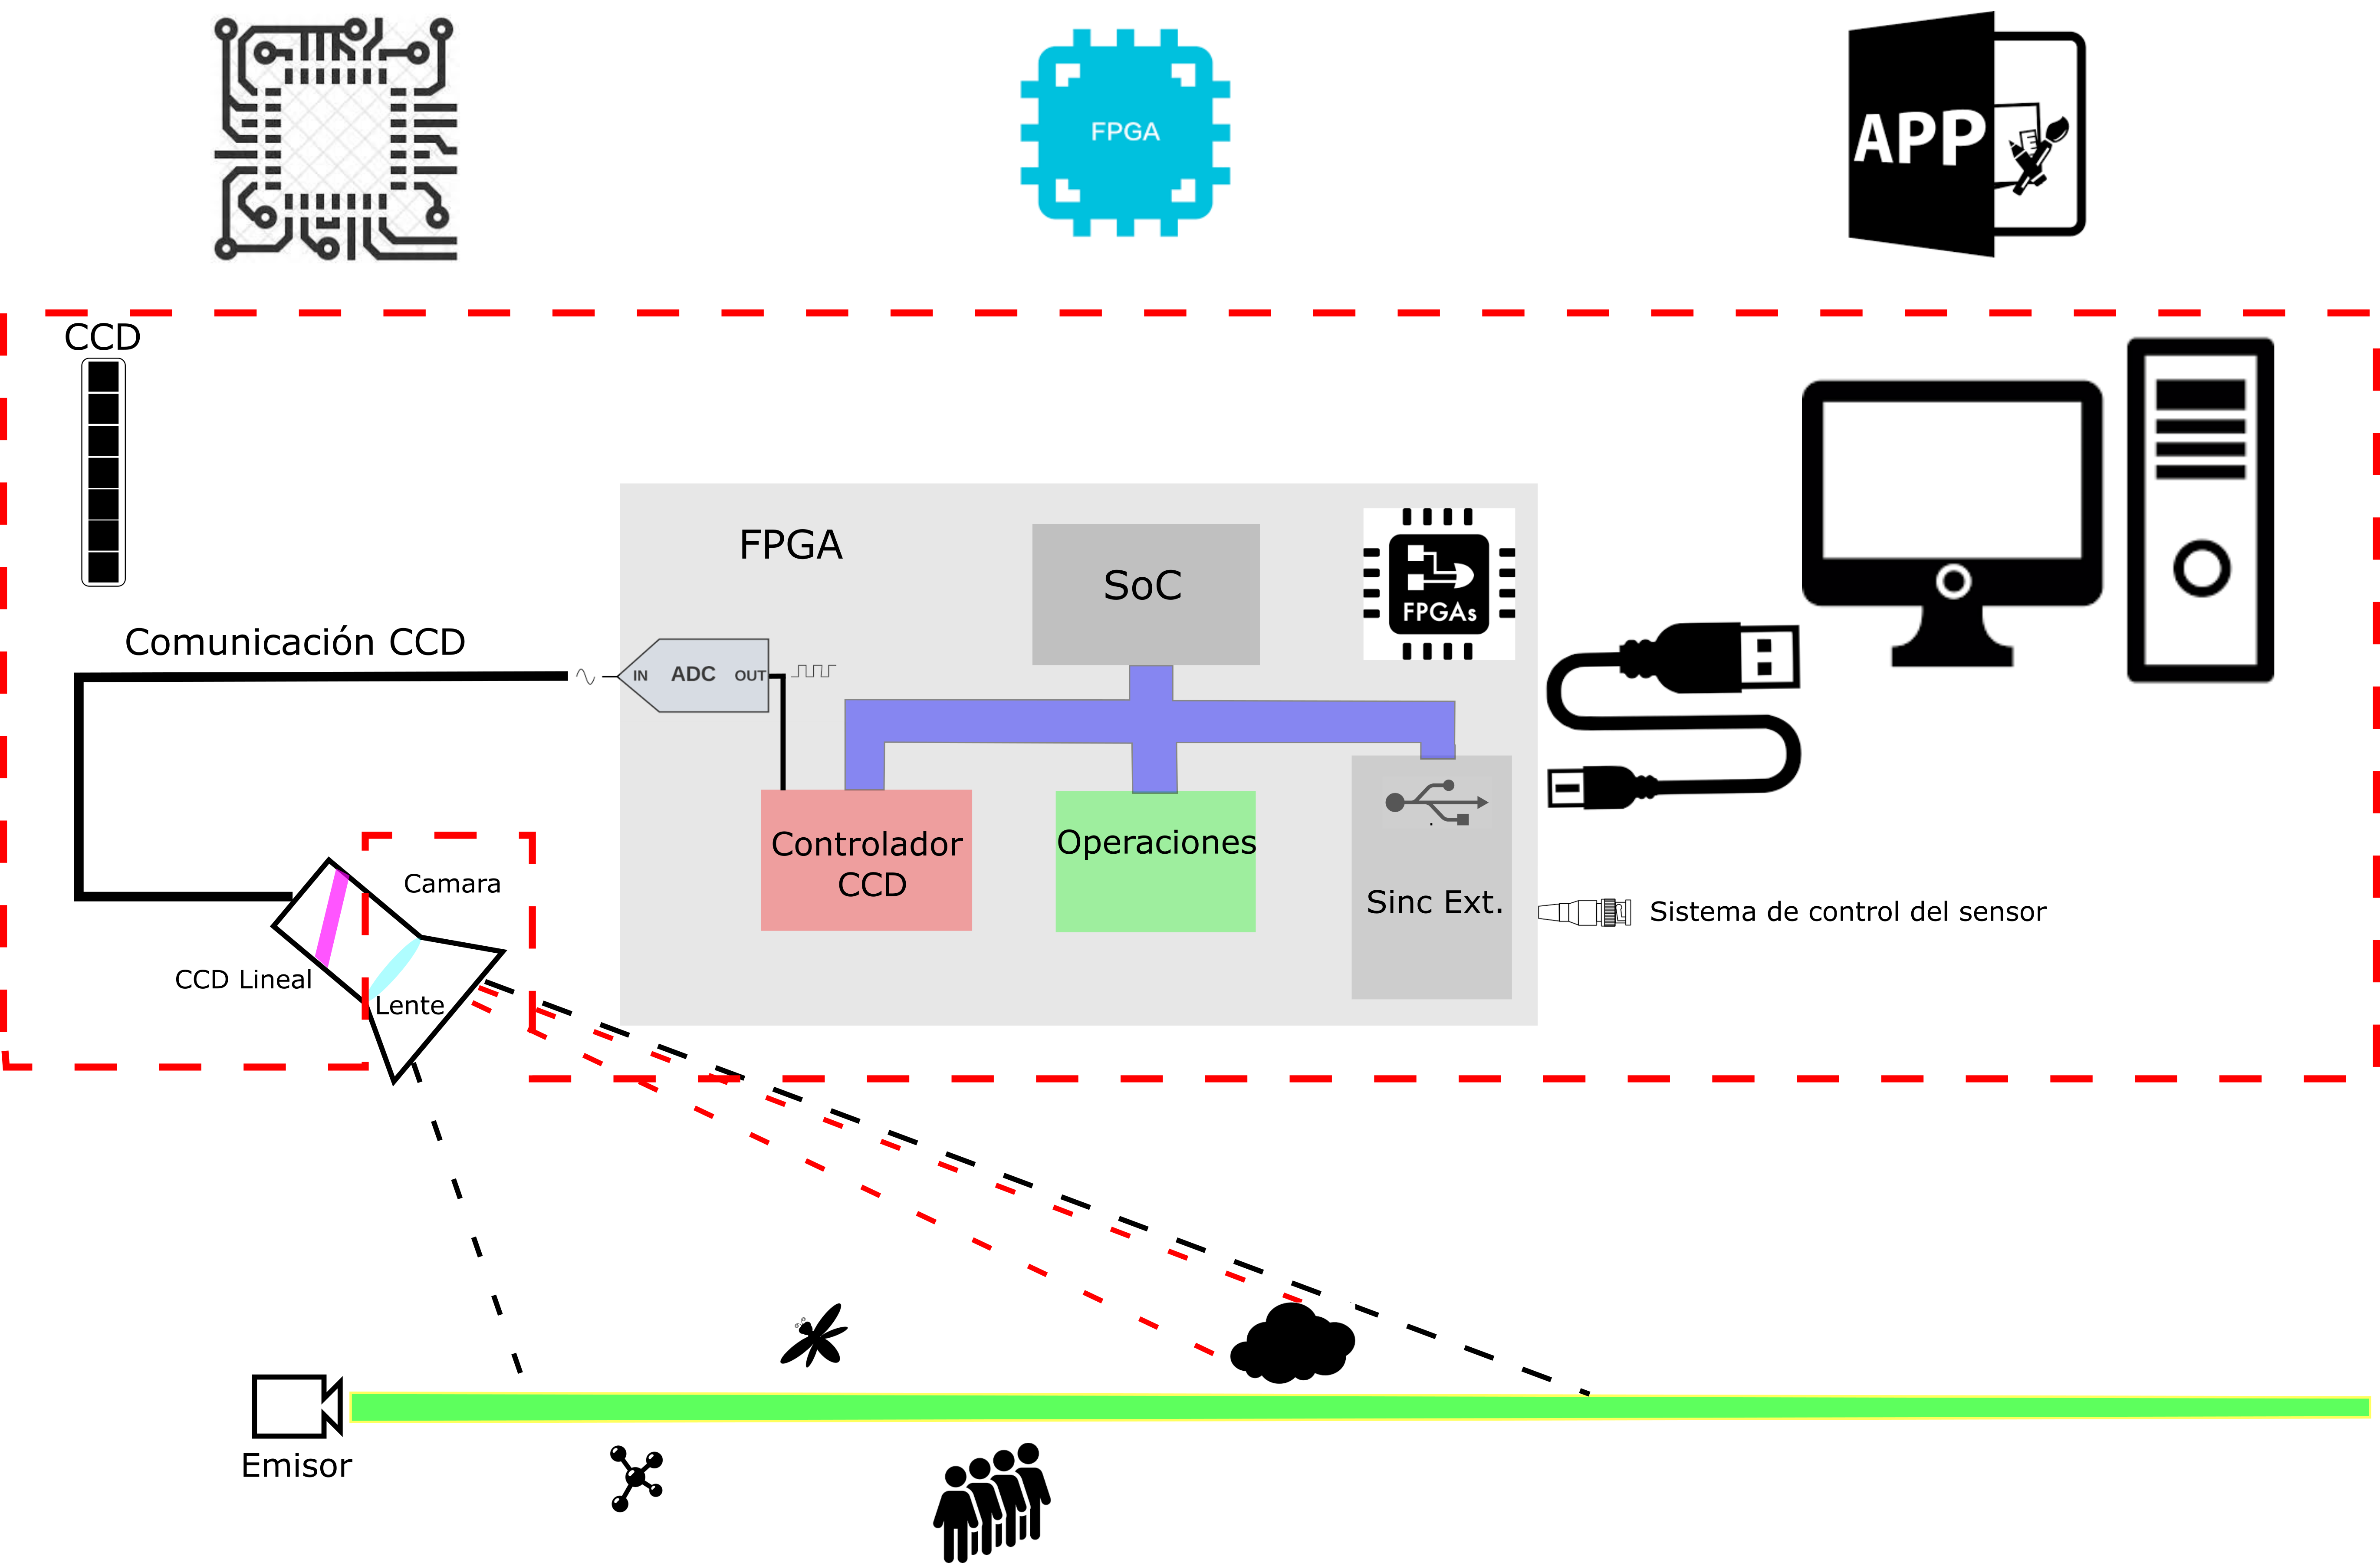
\includegraphics[width=.9\textwidth]{./Figuras/esquema_png.png}
\caption{Diagrama en bloques del sistema. El área delimitada por la línea con guiones rojos representa el alcance de este proyecto}
\label{fig:diagBloques}
\end{figure}

%\vspace{25px}

La cámara utiliza un sensor de carga acoplada como sensor de la luz entrante a través de la lente. La información colectada se traduce en una imagen y un sistema compuesto por un conversor analógico digital y un conjunto  de compuertas lógicas programables es responsable de digitalizar la señal, controlar el sensor y realizar el procesamiento de datos. El dato procesado se envía a una aplicación en la computadora responsable de la recopilación y seguimiento de las mediciones. La continua adquisición de medidas en el tiempo construye un conjunto de imágenes dispuestas en un arreglo lineal de filas y columnas. 

En el mercado existen dispositivos que permiten controlar y adquirir imágenes con un sensor de cargas acopladas, pero son insuficientes cuando se desea hacer procesamiento de los datos en tiempo real y en el mismo dispositivo donde se generan los datos.

El presente proyecto se destaca especialmente por incorporar un módulo de procesamiento embebido en la unidad de control que permite hacer operaciones estadísticas y reducir carga de procesamiento en la computadora. Este concepto se relaciona con la definición de \textit{Edge Computing}, donde el procesamiento se realiza cerca del origen de los datos. Esta característica nueva se diferencia de otros dispositivos en el mercado que hacen sus análisis una vez que la señal se almacenó, sin cumplir con requerimientos de procesamiento en tiempo real.





\section{2. Identificación y análisis de los interesados}
\label{sec:interesados}

\begin{consigna}{black} 


\begin{table}[ht]
%\caption{Identificación de los interesados}
%\label{tab:interesados}
\begin{tabularx}{\linewidth}{@{}|l|X|X|l|@{}}
\hline
\rowcolor[HTML]{C0C0C0} 
Rol           & Nombre y Apellido & Organización 	& Puesto 	\\ \hline
Auspiciante   & \clientename      & \empclientename             	& Jefe       	\\ \hline
Cliente       & \clientename      &\empclientename &	Jefe         	\\ \hline
Impulsor      & Dra Sandra Casas                  & UNPA-UARG      &  Directora ITA      	\\ \hline
Responsable   & \authorname       & CONICET        	& Alumno 	\\ \hline
Colaboradores & Esp. Ing Gonzalo Lavigna & FIUBA              	&Codirector        	\\ \hline
Orientador    & \supname	      & \pertesupname 	& Director Trabajo final \\ \hline
Equipo        & Ing. Jonathan Quiroga \newline 
			      Florencia Luna                                &  UNPA-UARG        	&  Investigador      	\\ \hline

Usuario final & Tec. Nahuel Diaz   &   CPA-CONICET   &  Técnico operador      	\\ \hline
\end{tabularx}
\end{table}



\end{consigna}



\section{3. Propósito del proyecto}
\label{sec:proposito}

\begin{consigna}{black}
El propósito de este proyecto es generar un diseño para control de un sensor de carga acoplada mediante la utilización de un arreglo de compuertas.

Se pretende lograr que el procesamiento intensivo de las señales se realice en el dispositivo de control a través de un sistema embebido que permita incrementar la integración y reducir la carga de procesamiento en la computadora. 

Las aplicaciones de este tipo de sensor en conjunto con un sistema óptico pueden cubrir un amplio rango de aplicaciones en el campo del sensado remoto.

Un objetivo adicional es lograr que el sistema sea escalable a otros sensores de la familia que se utilice.

\end{consigna}

\section{4. Alcance del proyecto}
\label{sec:alcance}

\begin{consigna}{black}
El presente proyecto incluye:

\begin{itemize}
	\item Diseño y elaboración de una placa de montaje superficial para instalar el sensor de imagen.
	\item Integración del hardware de control embebido en una placa FPGA.
	\item Selección del sensor de imagen según requerimientos del cliente
	\item Desarrollo del software para captura de datos y almacenamiento de la información en una computadora.
	\item Documentación

\end{itemize}

El presente proyecto no incluye especificaciones mecánicas de movimiento y manipulación del dispositivo.

\end{consigna}


\section{5. Supuestos del proyecto}
\label{sec:supuestos}


Para el desarrollo del presente proyecto se supone que:

\begin{itemize}
	\item Se contará con disponibilidad horaria
	\item Se contará con las herramientas de hardware y software desde el inicio del proyecto
	\item Se contará con el apoyo financiero durante todo el desarrollo
	\item Se contará con posibilidad de conseguir el sensor óptico y la placa FPGA
\end{itemize}


\section{6. Requerimientos}
\label{sec:requerimientos}

\begin{enumerate}
	\item Requerimientos diseño.
		\begin{enumerate}
			\item El sensor lineal se conecta en un PCB con componente superficiales.
			\item La placa con el sensor se debe conectar con el sistema embebido por un cable flexible.
		\end{enumerate}
		
	\item Requerimientos del sistema embebido
		\begin{enumerate}
			\item El sistema debe poder adquirir un mínimo de 50 líneas por segundo.
			\item El controlador embebido genera las señales de control y datos hacia el sensor de imágenes.
			\item Un SoC es el responsable del flujo de datos dentro de la FPGA y hacia la PC.
			\item El sistema embebido debe calcular las métricas estadísticas: mediana, rango intercuartil, máximos y mínimos de los datos enviados por el sensor de imagen.
			\item Tiempo mínimo de integración igual a 2 milisegundo.
			\item El sistema debe enviar los datos calculados a un PC por USB.
		\end{enumerate}
	\item Requerimientos de interfaz.
		\begin{enumerate}
			\item Se debe poder configurar el tiempo de integración en milisegundos (mínimo 2 ms) desde una interfaz en PC.
			\item La interfaz debe mostrar la señales con sus métricas estadísticos en tiempo real.
		\end{enumerate}
	\item Requerimientos de documentación.
		\begin{enumerate}
			\item El proyecto se documenta con control de versiones.
		\end{enumerate}
	\item Requerimiento de testing.
	\begin{enumerate}
			\item Se debe aplicar un filtro para bloquear la luz en la mitad del sensor y el resto sea pasante. Con mediciones continuas se verifica resultado en la PC.
			\item Firmware se caracteriza por uso de testbench en Vivado-SDK combinado con herramienta ILA Debugging.
		\end{enumerate}
	
\end{enumerate}


\section{7. Historias de usuarios (\textit{Product backlog})}
\label{sec:backlog}
Las historias se evalúan mediante tres niveles bajo, medio y alto representado por una escala entera entre 1 y 5. El puntaje de la historia se calcula como el valor más cercano a la serie de Fibonacci de su suma.

\begin{itemize}
\item \textbf{Como:} cliente. 
\item \textbf{Quiero:} que la adquisición de imágenes tenga la posibilidad de realizar análisis de los datos en el sistema embebido
\item \textbf{Para:} disminuir la carga de cálculo en la PC.
\begin{itemize}
\item Dificultad: alta (5) porque los ejemplos son muy escazos y casi nada en el campo de las FPGA.
\item Complejidad: media (3) la complejidad es media, se puede simular facilmente en cualquier lenguaje.
\item Riesgo: media (5) es un proceso que nunca se hizo.
\item Story point: $5+3+5\;=\;13$.
\end{itemize}
\end{itemize}

\begin{itemize}
\item \textbf{Como:} usuario final.
\item \textbf{Quiero:} que el programa pueda correr en sistema operativo Windows 10 y Linux.
\item \textbf{Para:} tener posibilidad de elegir el tipo de PC a utilizar.
\begin{itemize}
\item Dificultad: baja (2) hay amplia cantidad de opciones.
\item Complejidad: media (3) la complejidad es media, muchos lenguajes de código abierto corren bajo Windows o Linux.
\item Riesgo: media (3) es un proceso que ya se realizó anteriormente.
\item Story point: $2+3+3\;=\;8$.
\end{itemize}
\end{itemize}


\begin{itemize}
\item\textbf{Como:} Responsable.
\item \textbf{Quiero:} Tener comunicación con mi equipo, orientador y colaborador.
\item \textbf{Para:}comunicar los problemas que aparezcan.
\begin{itemize}
\item Dificultad: baja (3) media se planea cada dos semanas tener comunicación.
\item Complejidad: baja (1) la complejidad es baja. Se realiza en forma virtual.
\item Riesgo: baja (1) es un proceso que ya se realizó muchas veces.
\item Story point: $3+1+1\;=\;5$.
\end{itemize}
\end{itemize}

\section{8. Entregables principales del proyecto}
\label{sec:entregables}

\begin{consigna}{black}

Los entregables del proyecto son:

\begin{itemize}
	\item Manual de uso.
	\item Diagrama de circuitos esquemáticos.
	\item Código fuente del firmware y testbench.
	\item API del software para integrar con diferentes sensores.
	\item Informe final.
\end{itemize}

\end{consigna}

\section{9. Desglose del trabajo en tareas}
\label{sec:wbs}


\begin{enumerate}
\item Preparación entorno de trabajo (50 hs).
	\begin{enumerate}
	\item Búsqueda de bibliografía sobre sistemas similares (20 hs).
	\item Búsqueda de materiales (20 hs).
	\item Instalación herramientas de trabajo (10 hs).
	\end{enumerate}

\item Diseño placa sensor de imágenes y controlador (155 hs).
	\begin{enumerate}
	\item Esquemático de circuitos para elaboración PCB con componentes de montaje superficial para sensor de imagen (25 hs).
	\item Selección de componentes (10 hs).
	\item Ruteo de placa (35 hs).
	\item Verificación de diseño por colaboradores (20 hs).
	\item Diseño controlador en sistema embebido (40 hs).
	\item Desempeño del controlador mediante banco de pruebas (20 hs).
	\item Consulta con los supervisores del trabajo (5 hs).
	\end{enumerate}

\item Evaluación PCB módulos sensor de imágenes (65 hs)
	\begin{enumerate}
	\item Interconexión del módulo sensor de imágenes con FPGA (20 hs).
	\item Evaluar comunicación entre sensor y FPGA (20 hs).
	\item Enviar datos prueba desde el sistema embebido a la PC (20 hs).
	\item Consulta con los supervisores del trabajo (5 hs).
	\end{enumerate}

\item Módulo de cálculo estadístico embebido y comunicación (145 hs).
	\begin{enumerate}
	\item Estudiar una forma óptima y eficiente de implementar operaciones estadísticas (20 hs).
	\item Incorporar un SoC y controlar el flujo de datos entre bloques (40 hs).
	\item Implementar cálculo de valores estadístico en paralelo (20 hs).
	\item Integración de bloques (20 hs).
	\item Comunicación USB hacia la PC (40 hs).
	\item Consulta con los supervisores del trabajo (5 hs).
	\end{enumerate}	

\item Interfaz (105 hs).
	\begin{enumerate}
	\item Desarrollo de interfaz en Python para control del sensor y del sistema embebido (tiempo de integración, frecuencia de trabajo, visualización de señales) (40 hs).
	\item Documentación de código (20 hs).
	\item Integración de bloques (40 hs).
	\item Consulta con los supervisores del trabajo (5 hs).	
	\end{enumerate}		

\item Gestión (100 hs).
	\begin{enumerate}
	\item Planificación del trabajo final (15 hs).
	\item Informes regulares de avances (10 hs).
	\item Confección de la memoria de trabajo (45 hs).
	\item Presentación y defensa del trabajo final (20 hs).
	\item Consulta con los supervisores del trabajo (10 hs).
	\end{enumerate}		
\end{enumerate}

Cantidad total de horas: (620 hs)


\section{10. Diagrama de Activity On Node}
\label{sec:AoN}



\begin{figure}[htpb]
\centering 
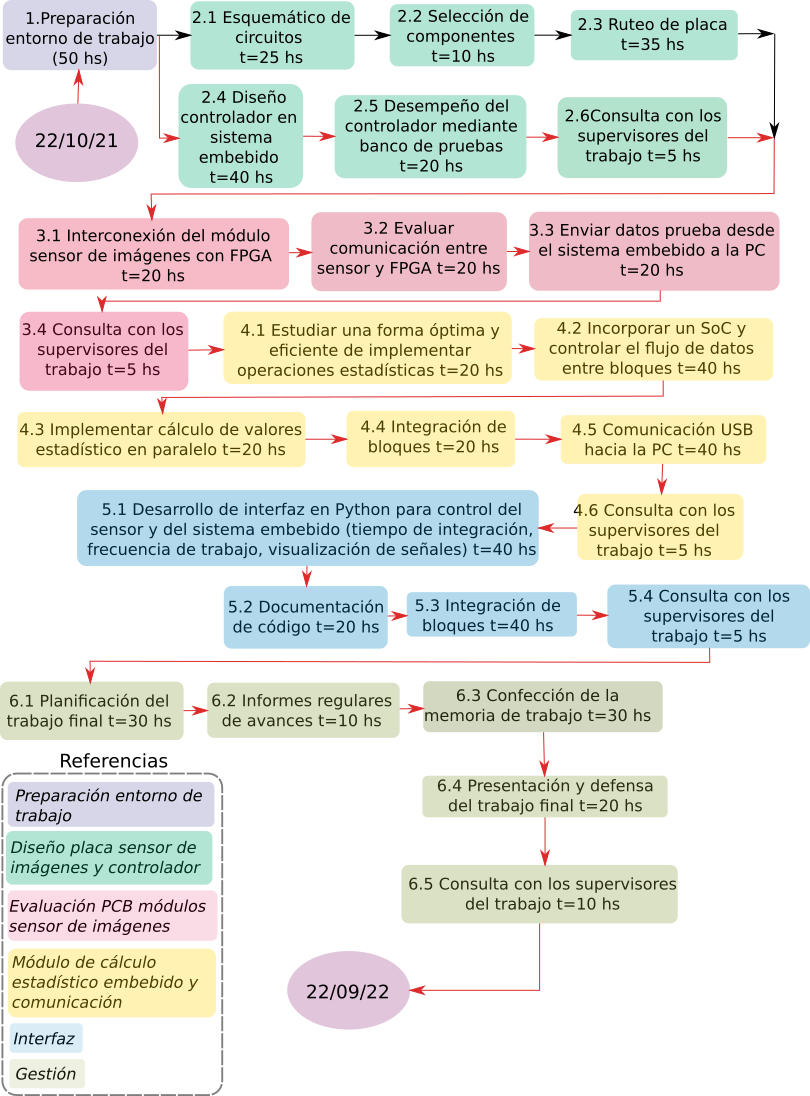
\includegraphics[width=.95\textwidth]{./Figuras/AoN2.png}
\caption{Diagrama en \textit{Activity on Node}}
\label{fig:AoN}
\end{figure}



\section{11. Diagrama de Gantt}
\label{sec:gantt}


\begin{landscape}
\begin{figure}[htpb]
\centering 
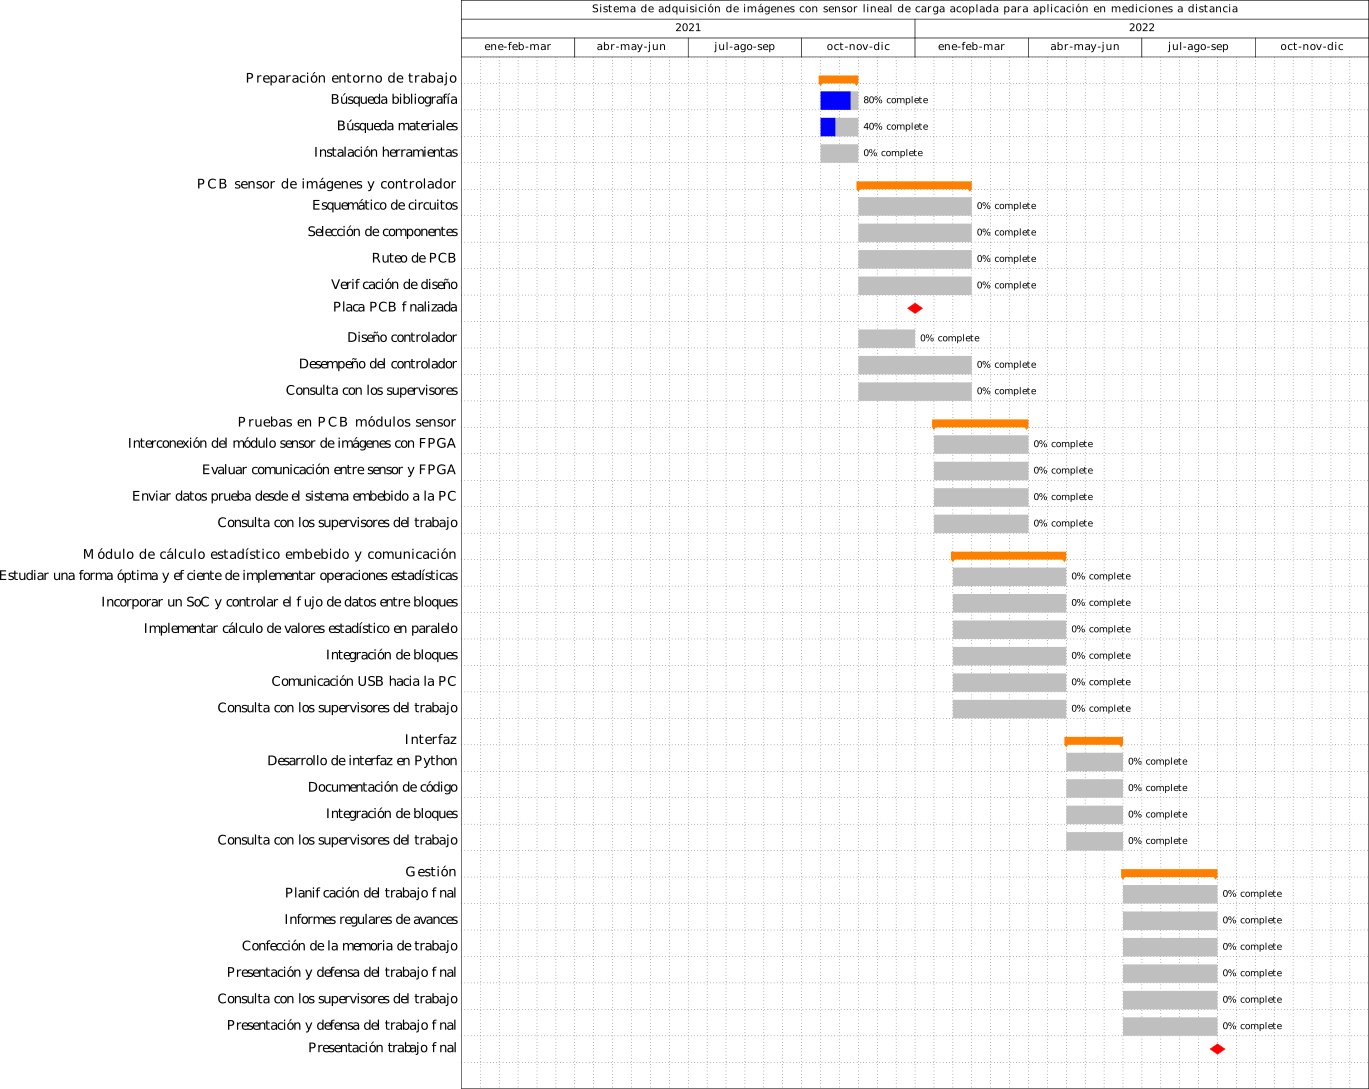
\includegraphics[height=.95\textheight]{./Figuras/gantt.png}
\caption{Diagrama de Gantt.}
\label{fig:diagGantt}
\end{figure}
\end{landscape}


%Comienzo de nueva pagina
%\pagebreak


\section{12. Presupuesto detallado del proyecto}
\label{sec:presupuesto}

\begin{table}[htpb]
\centering
\begin{tabularx}{\linewidth}{@{}|X|c|r|r|@{}}
\hline
\rowcolor[HTML]{C0C0C0} 
\multicolumn{4}{|c|}{\cellcolor[HTML]{C0C0C0}COSTOS DIRECTOS} \\ \hline
\rowcolor[HTML]{C0C0C0} 
Descripción &
  \multicolumn{1}{c|}{\cellcolor[HTML]{C0C0C0}Cantidad} &
  \multicolumn{1}{c|}{\cellcolor[HTML]{C0C0C0}Valor unitario} &
  \multicolumn{1}{c|}{\cellcolor[HTML]{C0C0C0}Valor total} \\ \hline
 Sensor de imágenes&
  \multicolumn{1}{c|}{1} &
  \multicolumn{1}{c|}{\$ 27.000} &
  \multicolumn{1}{c|}{ \$ 27.000} \\ \hline
 Placa de desarrollo FPGA &
  \multicolumn{1}{c|}{1} &
  \multicolumn{1}{c|}{\$ 45.000} &
  \multicolumn{1}{c|}{\$ 45.000} \\ \hline
Elaboración PCB &
\multicolumn{1}{c|}{1} &
  \multicolumn{1}{c|}{\$ 10.000} &
  \multicolumn{1}{c|}{\$ 10.000} \\ \hline
Componentes  &
\multicolumn{1}{c|}{varios} &
  \multicolumn{1}{c|}{\$ 20.000} &
  \multicolumn{1}{c|}{\$ 20.000} \\ \hline  
  

\multicolumn{3}{|c|}{SUBTOTAL} &
  \multicolumn{1}{c|}{\$ 102.000} \\ \hline
\rowcolor[HTML]{C0C0C0} 
\multicolumn{4}{|c|}{\cellcolor[HTML]{C0C0C0}COSTOS INDIRECTOS} \\ \hline
\rowcolor[HTML]{C0C0C0} 
Descripción &
  \multicolumn{1}{c|}{\cellcolor[HTML]{C0C0C0}Cantidad} &
  \multicolumn{1}{c|}{\cellcolor[HTML]{C0C0C0}Valor unitario} &
  \multicolumn{1}{c|}{\cellcolor[HTML]{C0C0C0}Valor total} \\ \hline
\multicolumn{1}{|l|}{Hora de ingeniería} &
    620 hs&
   \$ 1500&
   \$ 930.000
   \\ \hline


\multicolumn{3}{|c|}{SUBTOTAL} &
  \multicolumn{1}{c|}{\$ 930.000} \\ \hline
\rowcolor[HTML]{C0C0C0}
\multicolumn{3}{|c|}{TOTAL} &
   \$ 1.032.000\\ \hline
\end{tabularx}%
\end{table}


\section{13. Gestión de riesgos}
\label{sec:riesgos}


Riesgo 1: no conseguir el sensor de imágenes que cumpla con los requerimiento funcionales.
\begin{itemize}
	\item Severidad (S): 8(ocho) la severidad es alta. Pocas alternativas comerciales cumplen con los requerimientos funcionales.\\
	
	\item Probabilidad de ocurrencia (O): 4(cuatro) la probabilidad es relativamente baja, ya se envió orden de compra del sensor.
\end{itemize}  
 
 
Riesgo 2: no disponer de un kit de desarrollo de lógica programable.
\begin{itemize}
	\item Severidad (S): 2(dos) la severidad es baja ya  se dispone de kit para comenzar el trabajo.\\
	\item Probabilidad de ocurrencia (O): 5(cinco) la probabilidad es media. Existen al menos 4 proveedores confirmados con stock disponible de kit alternativos. 
\end{itemize}  


Riesgo 3: que el kit de desarrollo que se posee no cuente con los recursos de sintetizar el sistema general.
\begin{itemize}
	\item Severidad (S): 7(siete)  es alta. La gestión de compra y envió afecta la severidad.
	\item Ocurrencia (O): 5 (cinco) es media. El kit adecuado se descarta o selecciona con los resultados del programa de síntesis.
\end{itemize}

Riesgo 4: falta de tiempo para adquirir conocimientos para implementar todos los requerimientos.

%Se prestará especial atención al cumplimiento de los requerimientos técnicos desde el inicio de la %etapa de implementación especialmente en el manejo de la cantidad de canales de entrada.
\begin{itemize}
	\item Severidad (S): 7(siete) ss alta. Puede tener impacto en la calidad del proyecto final.
 
\item Ocurrencia (O): 2 (baja) es baja se cuenta con colaboradores para consultar con experiencia. 
\end{itemize}

Riesgo 5: no cumplir con los plazos establecidos. Se trabajará en base a la planificación prestando especial interés a la etapa 3 de metodologías y desarrollo.
\begin{itemize}
	\item Severidad (S): 7 (siete) la severidad es media ya que es un prototipo de desarrollo, existe parcialmente  bibliografía al respecto.\\
	\item Probabilidad de ocurrencia (O): 8 (ocho) es alta ya que el desarrollador responsable  cuenta con  experiencia parcial en desarrollo sobre dispositivos lógicos programables.

\end{itemize}  



b) Tabla de gestión de riesgos:      (El RPN se calcula como RPN=SxO)

\begin{table}[htpb]
\centering
\begin{tabularx}{\linewidth}{@{}|X|c|c|c|c|c|c|@{}}
\hline
\rowcolor[HTML]{C0C0C0} 
Riesgo & S & O & RPN & S* & O* & RPN* \\ \hline
No conseguir el sensor de imágenes que cumpla con los requerimientos funcionales.       & 8  &4   &32     &8    &4    &32      \\ \hline
No disponer de un kit de desarrollo de lógica programable.       &2   &5   & 10    &2    &5    &10     \\ \hline
El kit de desarrollo no cuente con los recursos de sintetizar el sistema general.       &7   &5   &35     &7    & 3   &     21 \\ \hline
Falta de tiempo para adquirir conocimientos para implementar todos los requerimientos.       &7   &2   &14     &5    & 5   & 25     \\ \hline
No cumplir con los plazos establecidos.      &7   &8   &56     &7    &4    & 28     \\ \hline
\end{tabularx}%
\end{table}

Criterio adoptado: 
Se tomarán medidas de mitigación en los riesgos cuyos números de RPN sean mayores a 34.

Nota: los valores marcados con (*) en la tabla corresponden luego de haber aplicado la mitigación.

c) Plan de mitigación de los riesgos que originalmente excedían el RPN máximo establecido:
 
Riesgo 3: que el kit de desarrollo que se posee no cuente con los recursos de sintetizar el sistema general.
\begin{itemize}
\item Severidad (S): La severidad sigue siendo la misma.       
\item Probabilidad de ocurrencia (O): 3 (tres) La probabilidad de ocurrencia es baja. Se hacen consultas con colaboradores.
\end{itemize}
  

Riesgo 5: No cumplir con los requerimientos planteados. Plan de mitigación: Se irá verificando los requerimientos a medida que se vayan realizando las pruebas de verificación y control. Los requerimientos a satisfacer son requisitos de máxima.
\begin{itemize}
\item Severidad (S):5 (cinco) la severidad sigue siendo la misma.
\item Probabilidad de ocurrencia (O): 3 (tres) La probabilidad de ocurrencia baja los requerimientos se irán verificando en las etapas de pruebas. 

\end{itemize}


Riesgo 5:  No cumplir con los plazos establecidos.
\begin{itemize}
\item Mitigación: Considerando la fecha de inicio y finalización de la 5 Cohorte de MSE, se aprecia que
durante los meses de enero y febrero del 2021 no se dictarán clases. Por este motivo, es
posible incorporar más horas de trabajo.
\item Severidad: 10. No se realiza ninguna modificación sobre este factor respecto a lo que se ha
propuesto originalmente.
\item Probabilidad de ocurrencia (O): 4 (cuatro) Se irán verificando los tiempos según lo planificados y lo desarrollado para ir detectando posibles incrementos.


\end{itemize}  


\section{14. Gestión de la calidad}
\label{sec:calidad}


Req \#1: El sensor lineal se conecta en un PCB con componente superficiales.
\begin{itemize}
\item Verificación:comprobar que los encapsulados que se utilicen en el diseño del PCB sean SMD.
\item Validación: mostrarle vista 3D del PCB al cliente.
\end{itemize}

Req \#2: La placa con el sensor se debe conectar con el sistema embebido por un cable flexible.
\begin{itemize}
\item Verificación:cable de largo 30 cm. 
\item Validación: fotografía del cable flex conectado entre el sensor y FPGA.
\end{itemize}

Req \#3: El sistema debe poder adquirir un mínimo de 50 líneas por segundo.
\begin{itemize}
\item Verificación: especificación por medio de la  hoja de datos del sensor.
\item Validación: generación de archivos de datos con un tiempo de integración de 1/50 segundos. Se cuentas las imágenes  almacenadas y que sean igual a 50.
\end{itemize}


Req \#4: El controlador embebido genera las señales de control y datos hacia el sensor de imágenes.
\begin{itemize}
\item Verificación: comprobar que las señales enviadas son digitales.
\item Validación: se valida por medio de testbench y simulaciones.
\end{itemize}

Req \#5: Un SoC es el responsable del flujo de datos dentro de la FPGA y hacia la PC.
\begin{itemize}
\item Verificación: esquema descriptivos de cada bloque
\item Validación: se valida por medio de testbench y simulaciones.
\end{itemize}

Req \#6: El sistema embebido debe calcular las métricas estadísticas: mediana, rango intercuartil, máximos y mínimos de los datos enviados por el sensor de imagen.
\begin{itemize}
\item Verificación: algoritmo de simulación escrito en C.
\item Validación: se valida por medio de testbench y simulaciones en VHDL.
\end{itemize}

Req \#7: Tiempo mínimo de integración igual a 2 milisegundo.
\begin{itemize}
\item Verificación: tiempo de integración descripto por hoja de datos del sensor.
\item Validación: generación de archivos de datos con tiempo de integración de 2 ms. En un segundo debe adquirir 500 imágenes.
\end{itemize}

Req \#8: El sistema debe enviar los datos calculados a un PC por USB.
\begin{itemize}
\item Verificación: bloque descriptivo VHDL
\item Validación: se valida por medio de testbench y simulaciones en VHDL.
\end{itemize}

Req \#9: La interfaz debe mostrar la señales con sus métricas estadísticos en tiempo real.
\begin{itemize}
\item Verificación: pantalla en escala para cada señal.
\item Validación: captura de pantalla con visualización en tiempo real de las señales.
\end{itemize}

Req \#10: El proyecto se documenta con control de versiones. 
\begin{itemize}
\item Verificación: utilización de herramienta Git.
\item Validación: comentarios en GitHub.
\end{itemize}

Req \#10: se debe aplicar un filtro para bloquear la luz en la mitad del sensor y el resto sea pasante. Con mediciones continuas se verifica resultado en la PC.
\begin{itemize}
\item Verificación: dejar bloqueada 50\% del sensor.
\item Validación: las imágenes que se adquieren muestran el 50\% con valores nulos (bloque).
\end{itemize}

Req \#11: Firmware se caracteriza por uso de testbench en Vivado-SDK combinado con herramienta ILA Debugging.
\begin{itemize}
\item Verificación: código con control de versiones.
\item Validación: modelización y visualización de señales ModelSim/Vivado SDK con bloque ILA y VIO.
\end{itemize}

\section{15. Procesos de cierre}    
\label{sec:cierre}

\begin{itemize}
\item Pautas de trabajo que se seguirán para analizar si se respetó el Plan de Proyecto original.\\
Jacobo Salvador se encargará de actualizar la tabla WBS, que se comparará con la versión original para determinar si se cumplió con la planificación.

\item Identificación de las técnicas y procedimientos útiles e inútiles que se emplearon, y los problemas que surgieron y cómo se solucionaron.\\
 Finalizado el proyecto de dejará documentado las diferentes técnicas y procedimientos que se utilizaron.

\item Indicar quién organizará el acto de agradecimiento a todos los interesados, y en especial al equipo de trabajo y colaboradores.\\
 Jacobo Salvador se encargará de confeccionar los agradecimientos de los interesados e instituciones participantes.


\end{itemize}



\end{document}
